\chapter{The Insieme Runtime [Peter]} \label{cap:runtime}
\index{Runtime}

%%%%%%%%%%%%%%%%%%%%%%%%%%%%%%%%%%%%%%%%%%%%%%%%%%%%%%%%%%%%%%%%%%%%%%%%%%%%%%%
%%%%%%%%%%%%%%%%%%%%%%%%%%%%%%%%%%%%%%%%%%%%%%%%%%%%%%%%%%%%%%%%%%%%%%%%%%%%%%%
\section{Overview}
%%%%%%%%%%%%%%%%%%%%%%%%%%%%%%%%%%%%%%%%%%%%%%%%%%%%%%%%%%%%%%%%%%%%%%%%%%%%%%%
\subsection{Architecture}
Section \ref{sec:overview:runtime:components} gives an overview of the basic structure and most important components of the Insieme Runtime.

%%%%%%%%%%%%%%%%%%%%%%%%%%%%%%%%%%%%%%%%%%%%%%%%%%%%%%%%%%%%%%%%%%%%%%%%%%%%%%%
\subsection{Coding Standards}
In addition to the compiler coding standards \ref{sec:compiler:codingstandards} (as far as they are applicable to C), the runtime adds several other conventions that should be respected. These standards were created and ratified using the Insieme Runtime autocratic process.

\begin{enumerate}

\item \textbf{The insieme runtime is written in C99}. It should compile without warnings on any supported system, even when full warnings are enabled.

\item \textbf{Naming conventions}
\begin{enumerate}

\item \textbf{General}: Types and functions are named using the lowercase\_and\_underscores convention.

\item \textbf{Prefix}: All externally visible symbols should be prefixed with \srcCodeInl{irt\_}. (Except globals, see below)

\item \textbf{Abbreviation}: Use full names in types and abbreviations in methods operationg on them.\\
Example: \srcCodeInl{irt\_errcode irt\_wi\_delete(irt\_work\_item* wi);}

\item \textbf{Output Parameters}: Output parameters should be prefixed with \srcCodeInl{out_}. Parameters used for input and output should be prefixed with \srcCodeInl{inout_}. \\
Example: \srcCodeInl{irt\_errcode irt\_wi\_create(irt\_work\_item** out\_wi);}

\item \textbf{Typedefs}: Typedefs are good as long as they convey semantic information. However, \textbf{never} typedef a pointer. Whether some variable is a pointer or a data item should always be immediately obvious.
All IRT structures/unions should follow this scheme w.r.t. typedef:
\begin{srcCode}
typedef struct _irt_work_item {
	//...
} irt_work_item;
\end{srcCode}

\item \textbf{Globals}: Globals should always be prefixed with \srcCodeInl{irt\_g\_} and used sparingly.
\end{enumerate}

\item \textbf{Integer Types}:
Use the integer types defined in inttypes.h whenever a specific precision is
required, and \textbf{always} in basic IRT data structures.
E.g. use \srcCodeInl{int32} instead of int and \srcCodeInl{uint32} instead of unsigned.

\item \textbf{Error Handling}:
Error handling is performed using a combination of thread local error data and
signals. 

\item \textbf{Const}:
Use \srcCodeInl{const} whenever possible.

\item \textbf{Basic Data Structure Design}:
When designing basic data structures used throughout the IR, follow these
guidelines:
\begin{itemize}
\item The data structure should have a fixed, minimal size.
\item If required, the data structure should be easy to serialize and distribute
  over a network.
\item Keep the number of indirect memory accesses and redirections required to
  perform frequent operations to a minimum.
\end{itemize}
\end{enumerate}

%%%%%%%%%%%%%%%%%%%%%%%%%%%%%%%%%%%%%%%%%%%%%%%%%%%%%%%%%%%%%%%%%%%%%%%%%%%%%%%
\subsection{Source Code Organization}

The runtime is implemented as a set of headers only. This has the advantage of enabling the back-end compiler to more easily perform full optimization/inlining of small runtime functions. Additionally, it makes sure that each stand-alone program produced by the compiler can be run on any supported system, without the need to ship additional stand-alone libraries.

The main disadvantage of this approach is fact that the whole runtime system has to be compiled every time an application is compiled. However, since it is pure C, the time for this is insignificant on most modern systems.

Because of this approach, larger files are split in two: a \textbf{header file \texttt{*.h}} including data structures and function declarations, and a \textbf{corresponding implementation file \texttt{*.impl.h}}.

All widely used declarations are gathered in the file \texttt{declarations.h} to mitigate include order problems and simplify use. Utilities and other components are gathered in individual subdirectories, with their own \texttt{impl} subdirectory if necessary. Finally, \texttt{irt\_all\_impls.h} is a convenience header that includes all the implementation headers. 

%%%%%%%%%%%%%%%%%%%%%%%%%%%%%%%%%%%%%%%%%%%%%%%%%%%%%%%%%%%%%%%%%%%%%%%%%%%%%%%
\subsection{Options}
This section summarizes options used to custmize the runtime system. Some options need to be specified at compile-time as \srcCodeInl{#defines}, while others can be adjusted for each invocation without recompilation, usually by supplying some environmant variables.

\subsubsection{Compile-time}
Table \ref{tab:runtime:options:compile} summarizes the compile-time options available in the runtime. \textbf{Note}: when using the Runtime in Runtime-as-a-service mode, it is of paramount importance that both the program and the runtime are compiled using the same set of options.
\begin{table}[htbp] \small
	\centering
    \begin{tabular}{|p{4cm}|c|p{6cm}|r|}
        \hline
        Name                              & Type   & Semantics                                                                      & Default \\ \hline \hline
        IRT\_LOGGING                       & bool   & enables basic log file generation (insieme\_runtime.log)                                                                & true          \\ \hline
        IRT\_RUNTIME \_TUNING                & bool   & enables runtime tuning of parallel loop scheduling                                                                     & false         \\ \hline
        IRT\_RUNTIME \_TUNING\_EXTENDED       & bool   & enables extended runtime tuning of parallel loop scheduling                                                            & false         \\ \hline
        IRT\_ENABLE \_INSTRUMENTATION        & bool   & enables instrumentation of runtime objects                                                                             & false         \\ \hline
        IRT\_ENABLE\_REGION \_INSTRUMENTATION & bool   & enables instrumentation of user-defined regions (depends on IRT\_ENABLE\_INSTRUMENTATION, will be enabled automatically) & false         \\ \hline
        IRT\_SANE \_PARALLEL\_MAX             & uint64 & maximum amount of chunks a loop or splittable work item will be divided into                                           & 2048          \\ \hline
        IRT\_MAX \_CORES                     & uint64 & maximum amount of hardware threads supported by the system                                                             & 2048          \\ \hline
        IRT\_MAX \_WORKERS                   & uint64 & maximum number of workers that can be spawned                                                                          & 2048          \\ \hline
        IRT\_MAX \_WORK\_GROUPS               & uint32 & maximum number of work groups a single work item can be a member of                                                    & 4             \\ \hline
  \end{tabular}
	\caption{Insieme Runtime -- Compile-time Options}
	\label{tab:runtime:options:compile}
\end{table}

\subsubsection{Runtime}
Some options can be set independently for each run of the system, without recompilation. This is handled with environment variables, which are listed in table \ref{tab:runtime:options:environment}. The default values NCPU and CWD refer to the number of hardware threads in the system and the current working directory of the runtime respectively.

\begin{table}[htbp] \small
	\centering
    \begin{tabular}{|p{3cm}|c|p{7cm}|r|}
        \hline
        Name                              & Type   & Semantics                                                                                                       & Default       \\ \hline \hline
        IRT\_NUM \_WORKERS                 & uint   & sets the number of workers used                                                                                 & NCPU                \\ \hline
        IRT\_AFFINITY \_POLICY             & string & sets the affinity policy used to map workers to threads; examples: "IRT\_AFFINITY\_FILL", "IRT\_AFFINITY\_SKIP 2", "IRT\_AFFINITY\_FIXED 0,3,6,9" (with 4 workers)                                                         & IRT\_AFFINITY\_FILL \\ \hline
	IRT\_CPU \_FREQUENCY                & uint   & sets the clock frequency (numerical values given in MHz) of any cores the workers are mapped to, examples: "MIN", "MAX", "OS", "2400"  & OS        \\ \hline
        IRT\_INST \_OUTPUT\_PATH           & string & sets the output path for log files generated by instrumentation                                                 & CWD                 \\ \hline
        IRT\_INST \_WORKER\_EVENT \_LOGGING & bool   & if enabled, general events are logged in per-worker event logs                                                  & false               \\ \hline
	IRT\_INST \_BINARY\_OUTPUT          & bool    & if enabled, events are logged in binary format instead of human-readable text                                   & false               \\ \hline
	IRT\_INST \_WORKER\_EVENT \_TYPES    & string  & sets the event types that should be logged, separated by commas, i.e. WO,WI,WG,DI                               & WO,WI,WG,DI         \\ \hline
        IRT\_INST \_PAPI\_EVENTS           & string & list of papi events that should be measured, separated by colons; examples: examples: "PAPI\_TOT\_CYC:PAPI\_L1\_TCM", "PAPI\_L2\_DCM"                                                & none                \\ \hline
        IRT\_DEFAULT \_VARIANT               & uint32 & default variant of multiversioned WIs to select; if this variant is not available for a WI, variant 0 is chosen & 0                   \\ \hline
    \end{tabular}
	\caption{Insieme Runtime -- Environment Variables}
	\label{tab:runtime:options:environment}
\end{table} \note{add affinity ref in table}


%%%%%%%%%%%%%%%%%%%%%%%%%%%%%%%%%%%%%%%%%%%%%%%%%%%%%%%%%%%%%%%%%%%%%%%%%%%%%%%
%%%%%%%%%%%%%%%%%%%%%%%%%%%%%%%%%%%%%%%%%%%%%%%%%%%%%%%%%%%%%%%%%%%%%%%%%%%%%%%
\section{Following an Execution}
In this section, the basic steps that are performed at runtime startup, during program execution and during shutdown are discussed. The intent is to give an overview of everything that happens at these times, but not necessarily to go into detail regarding all the steps. For simplicity, the standalone runtime mode is used in this overview.

\begin{figure}[tb]
	\centering
	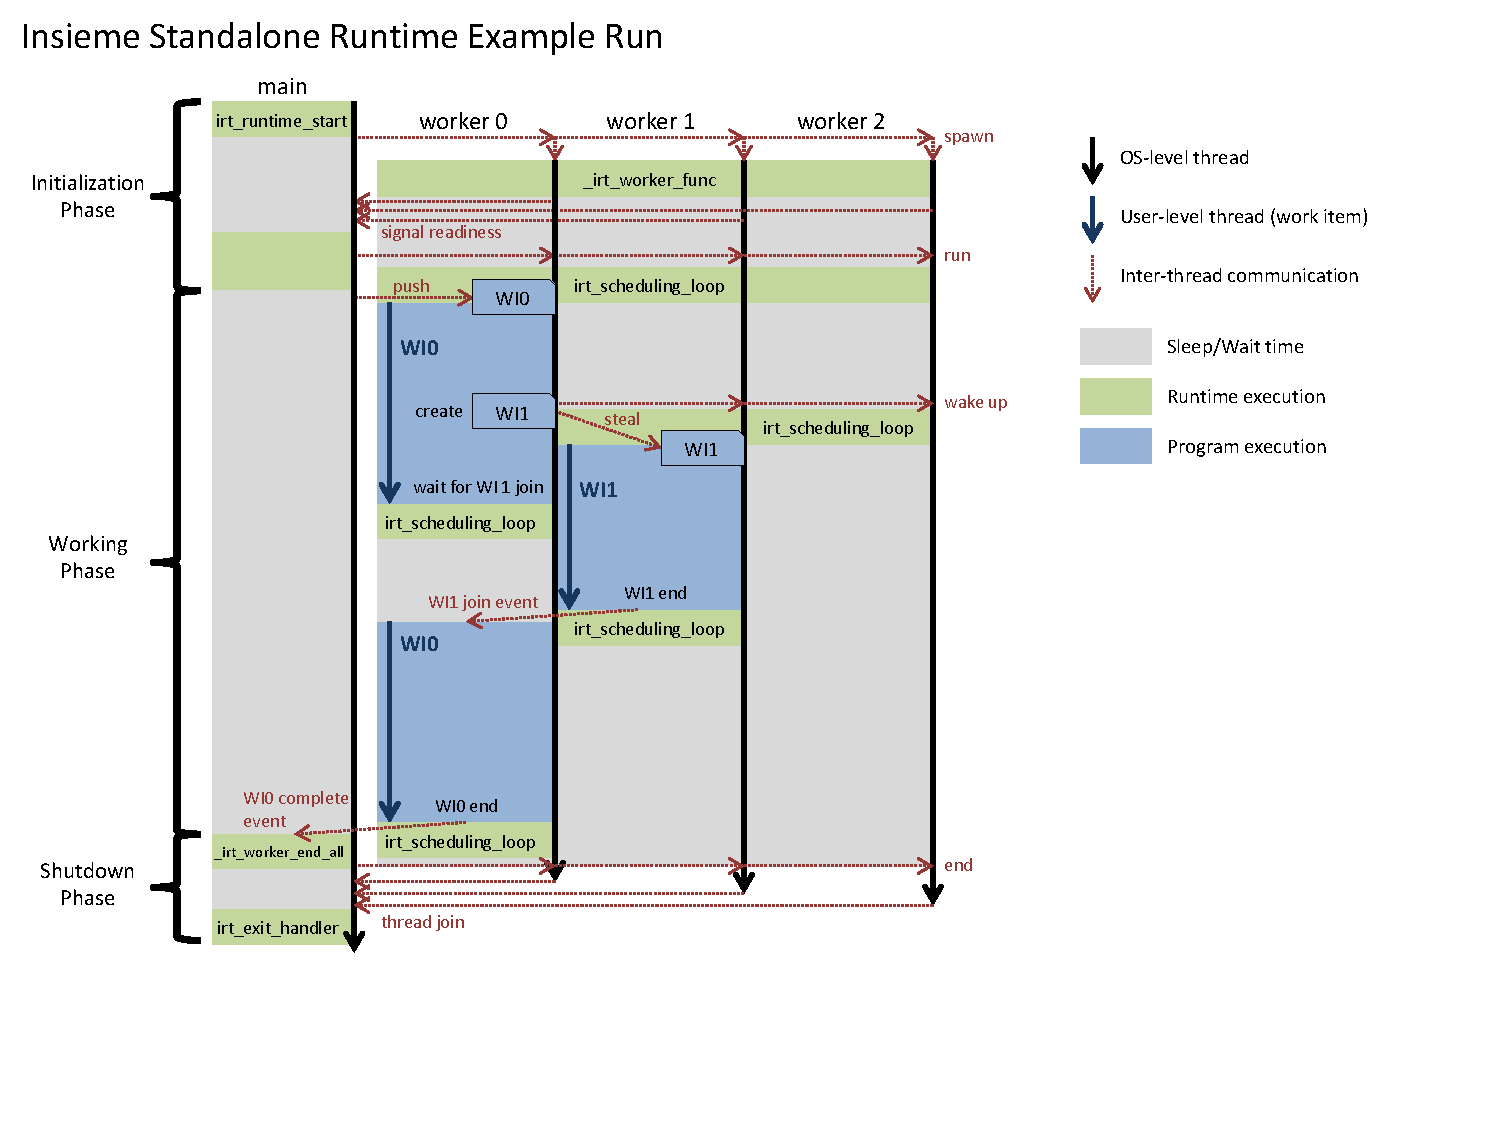
\includegraphics[width=\textwidth, trim=2cm 2cm 4cm 2cm]{pics/runtime/standalone_runtime_run.pdf}
	\caption{Timeline of a simple execution of the standalone runtime}
	\label{fig:runtime:execution}
\end{figure}


%%%%%%%%%%%%%%%%%%%%%%%%%%%%%%%%%%%%%%%%%%%%%%%%%%%%%%%%%%%%%%%%%%%%%%%%%%%%%%%
%%%%%%%%%%%%%%%%%%%%%%%%%%%%%%%%%%%%%%%%%%%%%%%%%%%%%%%%%%%%%%%%%%%%%%%%%%%%%%%
\section{Core}
\subsection{Workers}
\subsubsection{Scheduling}
\subsection{Work Items}
\subsection{Work Sharing}
\subsubsection{Loop Scheduling}
\subsection{Data Items}
\subsection{Event System}

\subsection{Instrumentation}
\label{sec:runtime.instrumentation}

\subsubsection{General Behaviour}
\label{sec:runtime.instrumentation.general.behaviour}

The instrumentation system of the runtime is used to get performance feedback
from the binaries generated by the compiler and executed with the runtime. It
generates two different kinds of performance data, one related to events in the
runtime (e.g. when was a work item created, started and ended) and one related
to code regions of the application program (e.g. how long did a code region run,
how efficient was its parallelism, how many floating point instructions did it
use).

The two different systems can be switched on and off for overhead and
pertubation reasons by defining \srcCodeInl{IRT_ENABLE_INSTRUMENTATION} (the
event-based instrumentation) and \srcCodeInl{IRT_ENABLE_REGION_INSTRUMENTATION}
(the region-based instrumentation) in instrumentation.h. Since the latter uses
some parts of the event instrumentation system, both of them must be switched on
for region-based instrumentation to work.

\subsubsection{Time measurements in the runtime}

Time measurements in the runtime are done as described in section
\ref{sec:runtime.abstraction.time.measurement}. During the execution of the runtime, all
performance data is logged in clock cycles. Any time-related performance data is
only converted to nanoseconds when it is written to a file. Since the writing is
done after the application has executed, this computational overhead will not be
measured.

\subsubsection{Event instrumentation system}

Note: Throughout this section, the abbreviations WI, WG, DI WO (or their
lower-case pendants) denote work item, work group, data item and worker.

The event instrumentation system can be enabled by defining
\srcCodeInl{IRT_ENABLE_INSTRUMENTATION} at compile time. To actually use it
during runtime, also either the environmental variable
IRT\_INST\_WORKER\_EVENT\_LOGGING needs to be set or instrumentation turned on
at a later point during runtime (described further below). If the system is
enabled and active, it will track the corresponding WI, WG, DI and worker events
together with the time they occurred and write this information to log files
when \srcCodeInl{irt_exit_handler} is called. The default path of these log
files is the current directory where the runtime is executed, unless a different
path was specified via IRT\_INST\_OUTPUT\_PATH. The files have the names
worker\_event\_log.NNNN where NNNN denotes the 4-digit number of the worker
thread which processed the event.

All event instrumentation functions are called via function pointers defined in
\file{instrumentation.impl.h}:

\begin{itemize} 
	\item \srcCodeInl{irt_inst_insert_wi_event} 
	\item \srcCodeInl{irt_inst_insert_wg_event} 
	\item \srcCodeInl{irt_inst_insert_wo_event} 
	\item \srcCodeInl{irt_inst_insert_di_event} 
\end{itemize}

The function pointers are either pointing to the corresponding instrumentation
functions (e.g. \srcCodeInl{_irt_inst_insert_wi_event()}) or are set to
empty functions (e.g. \srcCodeInl{_irt_inst_insert_no_wi_event()}. This way
of implementing allows for low-overhead switching between active and inactive
instrumentation during runtime. The toggling between active and inactive
instrumentation can be done via several functions that are provided solely for
this purpose:

\begin{itemize} 
	\item \srcCodeInl{irt_inst_set_wi_instrumentation(bool)} 
	\item \srcCodeInl{irt_inst_set_wg_instrumentation(bool)} 
	\item \srcCodeInl{irt_inst_set_wo_instrumentation(bool)} 
	\item \srcCodeInl{irt_inst_set_di_instrumentation(bool)} 
	\item \srcCodeInl{irt_inst_set_all_instrumentation(bool)} 
\end{itemize}


\section{Utilities} 
\subsection{Error Handling} 
\section{Abstraction}
\subsection{MinLWT -- Lightweight user-mode threads} 
\subsection{Affinity}
\subsection{Frequency switching} 

Frequency switching is done in \file{frequency.h}. It provides several functions for obtaining and setting the current processor frequency and currently only supports UNIX-based systems. The functions use settings in the CPU driver, thus this functionality depends on the driver's and the hardware's support of frequency swichting. The frequency settings of the CPU driver can be accessed at /sys/devices/system/cpu/cpu\textbf{N}/cpufreq/, where \textbf{N} denotes the core's id. Hence, for the runtime to be able to change the frequency, these device files must be readable and writable by the user executing the runtime.
%The following table lists the functions and their purpose:

%\begin{table}[htbp] \small
%	\centering
%	\begin{tabular}{|p{4cm}|c|p{6cm}|r|}
%        	\hline
%	        Name & Visibility & Semantics \\ \hline \hline
%		\srcCodeInl{int irt_cpu_freq_get_available_frequencies_core(irt_worker* worker, unsigned int** frequencies, unsigned int* length)} & external & Returns all possible frequencies supported by the core this worker runs on \\ \hline
%		\srcCodeInl{int _irt_cpu_freq_write(const char* path_to_cpufreq, const unsigned int frequency)} & internal & low-level function that sets a given driver setting to a given frequency \\ \hline
%		\srcCodeInl{int _irt_cpu_freq_read(const char* path_to_cpufreq)} & internal & low-level function that returns a given driver setting \\ \hline
%		\srcCodeInl{int irt_cpu_freq_get_cur_frequency_core(irt_worker* worker)} & external & Get the current frequency the core of a worker is running at \\ \hline
%		\srcCodeInl{int irt_cpu_freq_set_max_frequency_core(irt_worker* worker, unsigned int frequency)} & external & Set the maximum frequency the core of a worker is allowed to run at \\ \hline
%		\srcCodeInl{int irt_cpu_freq_set_min_frequency_core(irt_worker* worker, unsigned int frequency)} & external & Set the minimum frequency the core of a worker is allowed to run at \\ \hline
%		\srcCodeInl{int irt_cpu_freq_get_max_frequency_core(irt_worker* worker)} & external & Get the maximum frequency the core of a worker is allowed to run at \\ \hline
%		\srcCodeInl{int irt_cpu_freq_get_min_frequency_core(irt_worker* worker)} & external & Get the minimum frequency the core of a worker is allowed to run at \\ \hline
%		\srcCodeInl{int irt_cpu_freq_set_frequency_core(irt_worker* worker, unsigned int frequency)} & external & Set the frequency the core of a worker (by setting the minimum and the maximum to this value) \\ \hline
%		\srcCodeInl{int irt_cpu_freq_set_frequency(unsigned int frequency)} & external & Set the frequency of all cores of all workers (by setting the frequency for each core) \\ \hline
%		\srcCodeInl{int irt_cpu_freq_reset_frequency()} & external & Reset the minimum and the maximum frequencies of all cores of all workers to the system defaults \\ \hline
%		
%	\end{tabular}
%	\caption{Insieme Runtime frequency switching functions}
%	\label{tab:runtime:frequency}
%\end{table}

The frequencies are unsigned integers and given in MHz. For CPUs with vendor-supported overclocking (e.g. Intel Turbo Boost), Linux lists this mode as the maximum standard frequency + 1, i.e. 3401 MHz if the maximum clock frequency without overclocking is 3400 MHz. Hence, at the time of writing this documentation, such automatic overclocking features can only be enabled or disabled by the runtime, but not configured in detail.

\subsection{External Load measurement}

External load measurement is done in \file{load.h} and currently only supports UNIX-based systems. Process information from
/proc/self/stat and system information from /proc/stat is read by the functions
\srcCodeInl{get_load_own()} and \srcCodeInl{get_load_system()} respectively.
The latter returns two times, namely the time the system spent in syscalls and
the time the system was idle. Each function needs to be called twice to get an
actual measurement, since the system only provides current state information.
Hence, every call computes the load and stores the current system information
in static global variables defined in \file{load.h} to be used for the next
call. This implies that the first call to those functions will return invalid
numbers. The function \srcCodeInl{get_load_external()} provides the actual
external load by calling the former functions and dividing the values according
to the formula

\[ \text{external load} = \frac{\text{system time} - \text{runtime
time}}{\text{system time} + \text{idle time}} \].

Since the functions for obtaining external load are based on fscanf calls
parsing strings, and since external load readings for short time intervals are
likely not to be very useful due to noise, the interval between two
\srcCodeInl{get_load_external()} function calls should be at least around
100ms, depending on the system size.

\subsection{Time measurement} 
\label{sec:runtime.abstraction.time.measurement}

Note: all functions mentioned here can be found in \file{timing.h}.


Time measurements in the runtime are implemented using the x86-assembler rdtsc
instruction (and its pendant on powerpc architectures). Hence any time
measurements during the runtime's execution are only done in clock cycles, there
is no reference to real time in seconds. This has the advantage how both
providing low-overhead high-resolution and high-accuracy timers while at the
same time minimizing the overhead of converting these values to seconds (since
this will only be done when time measurements in seconds are actually required).
Any time-related data can be converted to nanoseconds by calling
\srcCodeInl{irt_time_convert_ticks_to_ns(uint64)} with the clock value as an
argument and using the return value.

Important to note is that rdtsc reads the TSC (time stamp counter) register of a
core. This register is only reset during a hardware reset or boot and counts
clock cycles while the processor is running. The registers between cores are not
synchronized between cores and therefore thread migration could lead to wrong
results. Since the runtime fixes the threads' affinity, this is not a problem.
Furthermore only relative times are of insterest, so small deviations between
the counters do not affect measurement results, considering the expected
lifetime of a single runtime execution. The presence of the TSC register and
whether it is constant over processor frequency changes can be checked with the
functions \srcCodeInl{irt_time_ticks_available()} and
\srcCodeInl{irt_time_ticks_constant()}. Currently, these functions are only
available for x86 processors.

The conversion between clocks and nanoseconds presumes that the ``clocks per
second'' ratio is available (and hence was calculated before). The runtime
achieves this by using \srcCodeInl{irt_time_ticks_per_sec_calibration_mark()},
which is called both at runtime startup/shutdown and which sets the global
variable \srcCodeInl{irt_g_time_ticks_per_sec}. Either this value is read from a
file \file{insieme\_reference\_cpu\_clocks} in the system's temporary directory,
or -- if the file is not present -- it is computed and saved to this file to be
available for any subsequent executions of the runtime. 

Thus, the first run on a freshly started system leads to this file being written
and any subsequent executions of the runtime will read this file rather than
re-compute the ratio. The function
\srcCodeInl{irt_time_ticks_per_sec_calibration_mark()} is called twice, at
runtime startup and shutdown. Both times it takes the time in clock cycles and
in real time using \srcCodeInl{gettimeofday()}, using the two respective
differences to compute the clocks per second. To ensure high accuracy, the
second call busy sleeps to increase the total execution time of the runtime to
at least 100 milliseconds if it executed faster than that. Hence, the first
execution of the runtime on a system without the calibration file in place will
have a minimum duration of 100ms.


\section{Customizing the Runtime}
